\section{Simulation Analysis}
\label{sec:simulation}

\subsection{Exercise 1}

Table~\ref{tab:Exercise1Simulation} shows the simulated operating point results for the circuit presented in Figure \ref{fig:CircuitDraw}. Again, currents designated below as $I_i$ refer to the currents passing through the respective resistances, $R_i$.

\begin{table}[H]
  \centering
  \begin{tabular}{|c|c|}
    \hline    
    {\bf Designation} & {\bf Value [A or V]} \\ \hline
    \input{../sim/Exercise1_tab.tex}
  \end{tabular}
  \caption{Operating point analysis table. Currents $I_i$ are in amperes; voltages $V_i$ are in volts.}
  \label{tab:Exercise1Simulation}
\end{table}

Comparing the theoretical analysis results presented in Table \ref{tab:Exercise1Theoretical} and the results in Table \ref{tab:Exercise1Simulation}, we can notice almost no differences. This was to be expected, since the circuit has no time dependency - meaning it's equal at any point in time. There is only a small difference between the two values of $I_c$, although it is negligible.\par
Now we ca approach the second point of our simulation where we see how the system behaves when $v_s(0)=0$ and the capacitor is replaced by a voltage souce $V_X$=V(6)-V(8), where the voltages are taken from \ref{tab:Exercise1Simulation}.

\begin{table}[H]
  \centering
  \begin{tabular}{|c|c|}
    \hline    
    {\bf Designation} & {\bf Value [A or V]} \\ \hline
    \input{../sim/Exercise2_tab.tex}
  \end{tabular}
  \caption{Operating point analysis table. Currents $I_i$ are in amperes; voltages $V_i$ are in volts.}
  \label{tab:Exercise2Simulation}
\end{table}

\subsection{Transient analisis}

Now we do a transient analisis of the values.

\begin{figure}[h] \centering
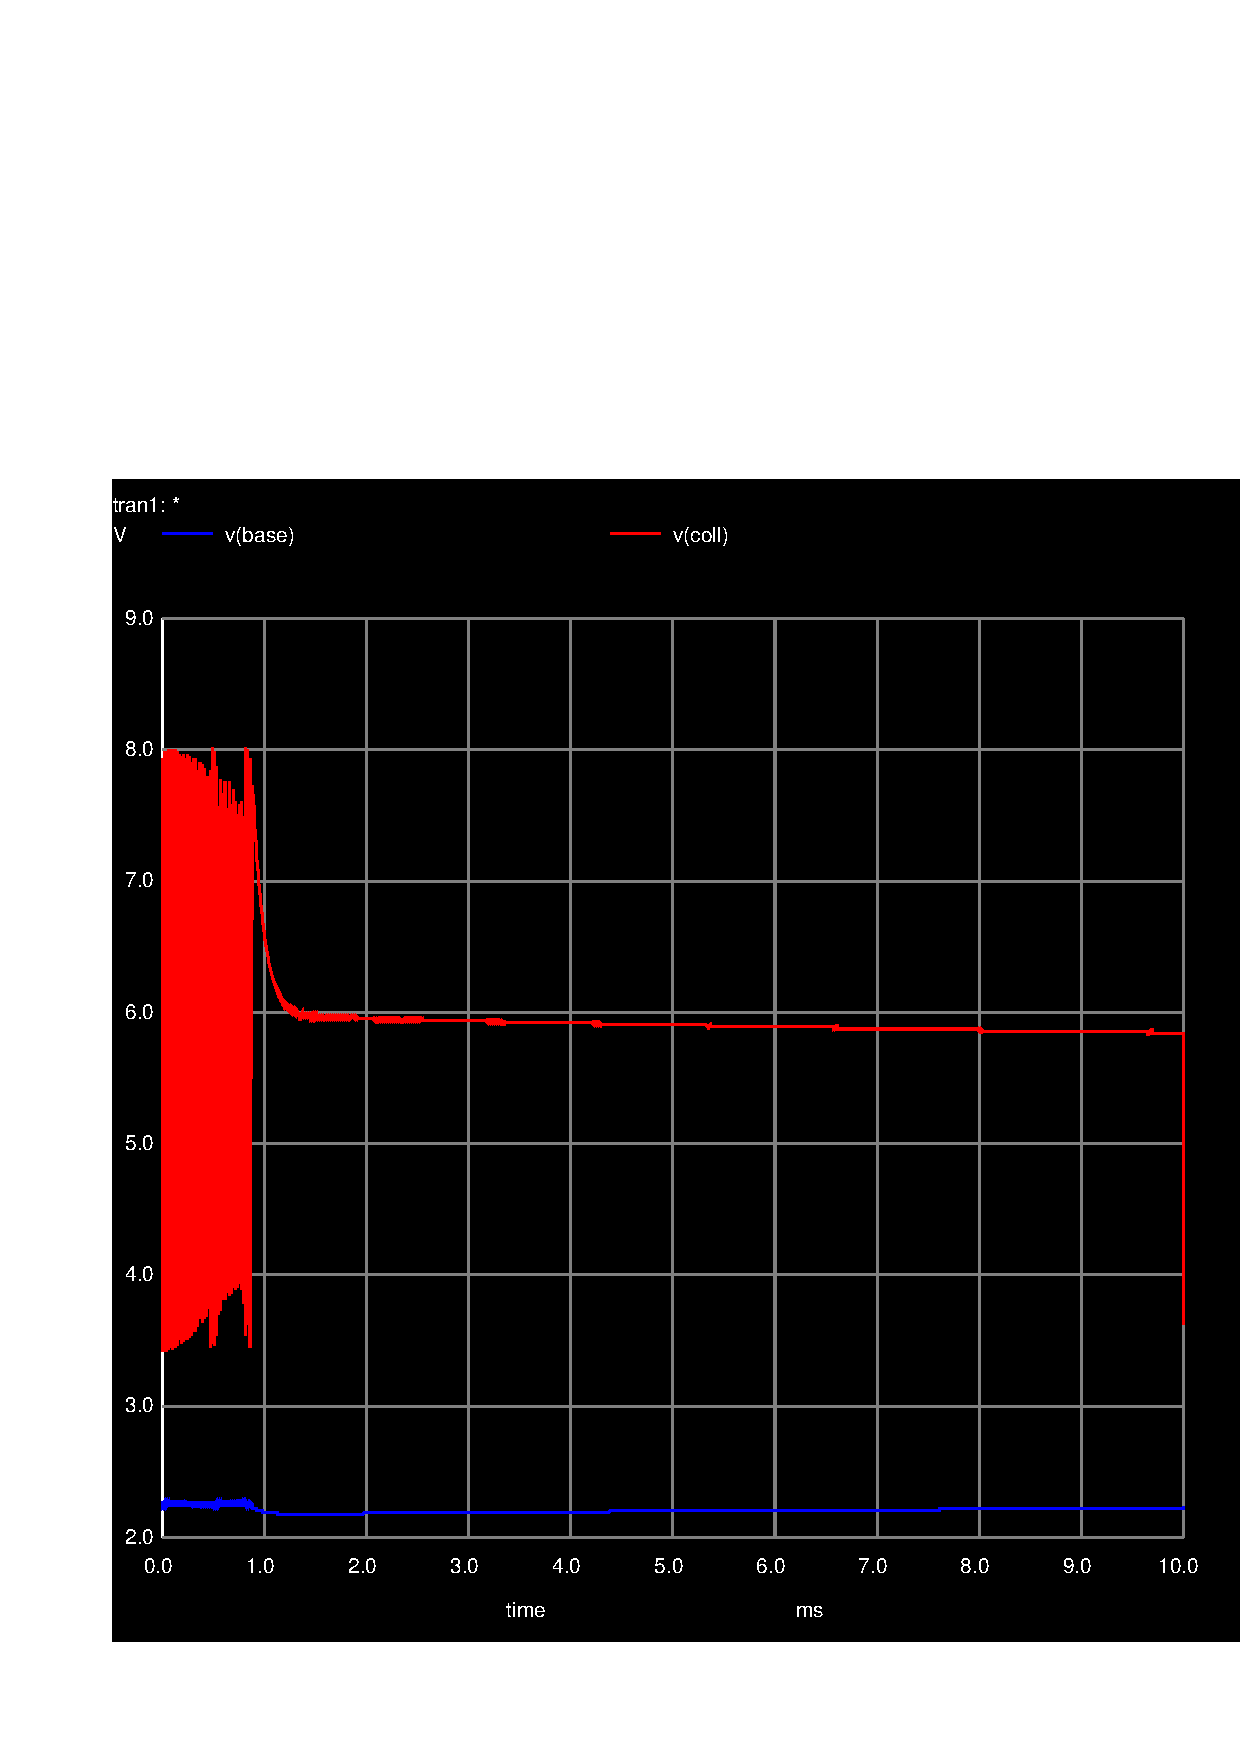
\includegraphics[width=0.8\linewidth]{../sim/trans.pdf}
\caption{Natural response.}
\label{fig:forced}
\end{figure}


\begin{figure}[h] \centering
\includegraphics[width=0.8\linewidth]{../sim/trans1.pdf}
\caption{Forced sinusoidal response and stimulus.}
\label{fig:forced}
\end{figure}
